\documentclass[10pt]{beamer}

\usepackage[utf8]{inputenc}
\usepackage[spanish]{babel}

\usepackage{graphicx}
\usepackage{multimedia}
\graphicspath{{./multimedia/}}

\usepackage{hyperref}

\immediate\write18{./Multimedia/tor\_status.sh > tor\_status.tex}
\immediate\write18{./Multimedia/tor\_flow.sh > tor\_flow.tex}

\usetheme[progressbar=frametitle]{metropolis}
\usepackage{appendixnumberbeamer}

\usepackage{booktabs}
\usepackage[scale=2]{ccicons}

\usepackage{pgfplots}
\usepgfplotslibrary{dateplot}

\usepackage{xspace}

\title{Tor(The onion router) y Riffle}
\subtitle{Protocolos de comunicación anónima}
\date{\today}
\author{Ignacio Aguilera Martos \and \\ Luis Balderas Ruiz}


\begin{document}
	

	
	
%Diapositiva de Título.
\frame{\titlepage}

%%%%%%%%%%%%%%%%%%%%%%%%%%%%%%%%%%%%%%%%%%%%%%%%%%%%%%%%%%%%%%%%%%%%%%%%%%%%%%%%%%%%%%%%%
%%%%%%%%%%%%%%%%%%%%%%%%%%%%%%%%%%%%Parte de Tor%%%%%%%%%%%%%%%%%%%%%%%%%%%%%%%%%%%%%%%%%
%%%%%%%%%%%%%%%%%%%%%%%%%%%%%%%%%%%%%%%%%%%%%%%%%%%%%%%%%%%%%%%%%%%%%%%%%%%%%%%%%%%%%%%%%
	
%Índice
\begin{frame}{Contenidos}
	\setbeamertemplate{section in toc}[sections numbered]
	\tableofcontents[hideallsubsections]
\end{frame}

%Sección que se incluye en el índice.
\section{Tor(The onion router)}

%Diapositiva de introducción de Tor.
\begin{frame}[fragile]{Propósito de Tor}
	%Lista de cosas que aparecen en diferentes páginas.
	\begin{itemize}
		\item<1-> Comunicaciones anónimas.
		\item<2-> $\boldsymbol{NO}$ se pretende respaldar a delincuentes.
		\item<3-> Es una red compleja de analizar.
	\end{itemize}
\end{frame}

%Diapositiva del esquema básico de Tor
\begin{frame}[fragile]{Esquema básico de Tor}
	\pause
	Las entidades básicas de Tor son:\pause
	\begin{itemize}
		\item<1-> Nodos.\pause
		\item<2-> Usuarios.\pause
		\item<3-> Autoridades de Directorio.
	\end{itemize}
	\pause
	\metroset{block=fill}
	%Bloque de alerta de información.
	\begin{alertblock}{Proxys y Tor}
		La relación entre nodos es similar a los proxys pero no es la misma.
	\end{alertblock}
\end{frame}

%Diapositiva acerca de los nodos.
\begin{frame}[fragile]{Nodos y sus tipos}
	\pause
	Los nodos son las piezas fundamentales de Tor.\\
	\pause
	Tipos: \pause
	\metroset{block=fill}
	%Bloque de definición.
	\begin{block}{Nodos Guard o Nodos de entrada}
		Son los nodos que ocupan el primer lugar en los circuitos. Son críticos ya que conocen la identidad del usuario.
	\end{block}
	\pause
	\begin{block}{Middle Nodes o Relay}
		Son los nodos intermedios dentro de los circuitos. Son los más básicos.
	\end{block}
	\pause
	\begin{block}{Exit Nodes o Nodos de salida}
		Son los nodos que ocupan el último lugar de los circuitos. Estos nodos tienen la información sin encriptar para enviarla al servidor de destino.
	\end{block}
\end{frame}

%Diapositiva acerca de los circuitos.
\begin{frame}[fragile]{Circuitos y su temporalidad}
	\pause
	\metroset{block=fill}
	\begin{block}{Circuito}
		Es un camino de nodos dentro del grafo de la red Tor. Incluye un nodo de entrada, varios nodos intermedios y un nodo de salida.
	\end{block}
	\pause
	Los circuitos tienen una caducidad (modificable por el usuario) por motivos de seguridad.
\end{frame}

%Diapositiva sobre los flags de los nodos.
\begin{frame}[fragile]{Flags de calificación de nodos}
	\pause
	\begin{itemize}
		\item<1-> BadExit.\pause
		\item<2-> Fast : 100KB/s.\pause
		\item<3-> Guard: 250KB/s. \pause
		\item<4-> Authority.\pause
		\item<5-> Exit.\pause
		\item<6-> HSDir: Hidden Service Directory.\pause
		\item<7-> Named o Unnamed.\pause
		\item<8-> Running: 45 minutos en ejecución.\pause
		\item<9-> Stable: 7 días en ejecución.\pause
		\item<10-> Valid: lista negra y versión de Tor sin alterar.\pause
		\item<11-> V2Dir\pause
	\end{itemize}
	\pause
	Gracias a estos flags los nodos quedan valorados para saber su posición en los circuitos y su validez como nodo en general.
\end{frame}

%Diapositiva acerca del ciclo de vida de un nodo.
\begin{frame}[fragile]{Ciclo de vida de un nodo}
	\pause
	Ocurre en 4 fases:
	\pause
	\begin{itemize}
		\item<1-> Fase 1(0-3): Comprobaciones básicas. Tests de seguridad y velocidad.\pause
		\item<2-> Fase 2(3-8): Nodo intermedio. Comprobaciones sobre Guard y Exit.\pause
		\item<3-> Fase 3(8-68): Nodo Guard. Comprobaciones de estabilidad y Exit.\pause
		\item<4-> Fase 4(68-...): Nodo Exit. Comprobaciones esporádicas generales.\pause
	\end{itemize}
\end{frame}

%Diapositiva sobre los servicios ocultos.
\begin{frame}[fragile]{Servicios Ocultos}
	\pause
	Los integrantes de esta comunicación son:
	\pause
	\begin{itemize}
		\item<1-> Usuario.\pause
		\item<2-> Servicio Oculto.\pause
		\item<3-> Puntos Introductorios.\pause
		\item<4-> Nodo Rendezvous.\pause
	\end{itemize}
	\pause
	\metroset{block=fill}
	\begin{block}{Diagrama de Comunicación}
		\footnotesize $Usuario \Leftrightarrow Guard \Leftrightarrow Relay \Leftrightarrow Rendezvous \Leftrightarrow Relay \Leftrightarrow Guard \Leftrightarrow Servicio \ oculto$
	\end{block}
	\pause
	\begin{exampleblock}{Direcciones Onion}
		Los servicios ocultos tienen URLs con el dominio onion y contienen 16 caracteres.\\ Por ejemplo: ab2dafgh1jklmi3t.onion ó facebookcorewwwi.onion.
	\end{exampleblock}
\end{frame}

%Diapositiva de Descriptores
\begin{frame}[fragile]{Descriptores}
	\pause
	\begin{itemize}
		\item<1-> Server Descriptor: IP, ORPort, ... \pause
		\item<2-> ExtraInfo Descriptor: Información completa del nodo. \pause
		\item<3-> Micro Descriptor: Información reducida del nodo. \pause
		\item<4-> Network Status Document: fichero de consenso.\pause
		\item<5-> Router Status Entry: Información completa de nodos incluyendo flags y cálculos heurísticos.\pause
		\item<6-> Hidden Service Descriptor: Información del servicio oculto.\pause
	\end{itemize}
\end{frame}

%Diapositiva de Puentes
\begin{frame}[fragile]{Puentes}
	\pause
	\metroset{block=fill}
	\begin{block}{Puente}
		Nodos ocultos usados para impedir las prohibiciones de uso de Tor por gobiernos o cualquier otra entidad.
	\end{block}
\end{frame}

%Diapositiva de Autoridades de Directorio.
\begin{frame}[fragile]{Autoridades de Directorio}
	\pause
	\metroset{block=fill}
	\begin{block}{Autoridad de Directorio}
		Nodo con permisos totales en la red. Son los únicos nodos de confianza. Tienen como misión controlar los nodos, valorarlos y administrar la red en general.
	\end{block}
\end{frame}

%Diapositiva de los ataque a Tor.
\begin{frame}[fragile]{Vulnerabilidades y fallos de diseño}
	\pause
	\metroset{block=fill}
	\begin{itemize}
		\item<1-> Correlación punto a punto.\pause
		\item<2-> Pérdida de información del nodo de salida.\pause
		\item<3-> Bloqueo de los nodos de salida.\pause
		\item<4-> Ataque DDOS a Tor.\pause
		\item<5-> HeartBleed.\pause
	\end{itemize}
\end{frame}

%%%%%%%%%%%%%%%%%%%%%%%%%%%%%%%%%%%Parte de Riffle%%%%%%%%%%%%%%%%%%%%%%%%%%%%%%%%%%%%%%%


\section{Riffle como solución}

%Diapositiva de introducción Riffle
\begin{frame}[fragile]{Introducción}
	\pause
	La aparición de un nuevo paradigma de comunicación segura y anónima se debe a: \pause
	\begin{itemize}
		\item<1-> El anonimato es un derecho fundamental en las sociedades democráticas. \pause
		\item<2-> Las Redes Tor son susceptibles ante ataques de análisis de tráfico. \pause 
		\item<3-> Alternativa: Redes que ofrecen resistencia al análisis del tráfico: DC-Nets y MixNets. \pause
		\item<4-> Dichas redes tienen problemas de eficiencia (Overhead de banda ancha y computacional).
	\end{itemize}
\end{frame}


%Diapositiva de presentación Riffle
\begin{frame}[fragile]{Presentación de Riffle}
	\pause
	Riffle: Sistema de comunicación anónima que garantiza el anonimato y minimiza los costes computacionales y de banda ancha. Prototipado por MIT en agosto de 2016. Propiedades: \pause
	\begin{itemize}
		\item<1-> Sistema híbrido de mezcla garantizada con encriptación simétrica. \pause
		\item<2-> Recuperación de información privada. \pause
		\item<3-> Eficientes comunicaciones anónimas resistentes al análisis del tráfico de datos como a clientes maliciosos. \pause
	\end{itemize}
\end{frame}

%Diapositiva Propiedades de seguridad
\begin{frame}[fragile]{Propiedades de seguridad}
	\pause
	\metroset{block=fill}
	\begin{block}{Definición 1}
		El protocolo es correcto si, después de una ejecución satisfactoria del protocolo,
		todo mensaje de un cliente honesto está
		disponible para todos los clientes honestos. \pause
	\end{block}	
	\begin{block}{Definición 2}
		El protocolo provee anonimato al emisor si, para toda ronda de comunicación, la probabilidad de que un adversario descubra el cliente honesto que mandó un mensaje es suficientemente cercana a $\frac{1}{k}$, siendo $k$ el número de clientes honestos. \pause
	\end{block}
	\begin{block}{Definición 3}
		El protocolo provee anonimato al receptor si, para toda ronda de comunicación, la probabilidad de que un adversario descubra el cliente honesto que mando un mensaje es suficientemente cercana a $\frac{1}{n}$, siendo $n$ el número de mensajes disponibles.
	\end{block}
\end{frame}	

\section{Arquitectura Riffle}

%Diapositiva Mezcla Híbrida Comprobable. No me cabe entero. Cómo se apaña???
\begin{frame}{Mezcla Híbrida Comprobable. Algoritmo}
	\pause
	\small{
		\begin{enumerate}
			\item \textbf{Compartir claves:} Un probador P y un verificador V generan parejas de claves públicas-privadas $(s_P,p_P)$ y $(s_V,p_V)$ y hacen públicas las claves $p_P$ y $p_V$. Un cliente C comparte sus claves $\{k'_i: i \in [n]\}$ con P.
			\item \textbf{Permutación de las claves:} C genera $\{k_i: i \in [n]\}$ para V y manda $\{Enc_{p_p}(Enc_{p_v}(k_j))\}$ a P y V. P desencripta y mezcla de
			forma verificada usando una permutación aleatoria $\pi$, y manda
			$\{Enc{p_v}(k_{\pi_j})\}$ a V. V verifica la mezcla y la desencriptación, y desencripta para ver $\{k_{\pi _j}\}$.
			\item  \textbf{Envío de mensajes:} Para $r=1,...,R,$
			\begin{enumerate}
				\item Mezcla: Para mandar mensajes $\{M_j^r\}_{j \in [n]}$ C encripta los mensajes en capas (onion-encrypt) y envía
				$\{AEnc_{k'_j,r}(A Enc_{k_j ,r}(M_j ^r))\}_{j \in [n]}$ a P, donde $AEnc$ es un esquema autenticado encriptado que usa r como nonce. P desencripta una capa de la encriptación usando $\{k'_j\}_{j \in [n]}$, los permuta usando la misma $\pi$ y manda $\{AEnc_{k_\pi(j),r}(M_{\pi(j)} ^r))\}_{j \in [n]}$ a V.
				\item Verificación: V verifica el texto cifrado comprobando la autenticación a través de las claves $\{k_{\pi(j)}\}_{j \in [n]}$ y r, desencripta una capa y adquiere los mensajes $\{M_{\pi(j)}^r\}_{j \in [n]}$.
			\end{enumerate}
		\end{enumerate}
	}
	
\end{frame}

%Diapositiva PIR

\begin{frame}{Recuperación de información privada. Algoritmo}
	\pause
\begin{enumerate}
	\item Configuración. Cada cliente $C_j$ comparte dos secretos $m_{i,j}$ y $s_{i,j}$  con cada servidor $S_i$ excepto con su servidor principal $S_{p_j}$. Esto pasa una vez por época.
	\item Descarga:
	\begin{enumerate}
		\item Generación de máscaras. Sea $I_j$ el índice del mensaje que $C_j$ quiere descargar. $C_j$ genera $m_{p_j,j}$ de forma que $\oplus _i m_{i,j} = e_{I_j}$, donde $e_{I_j}$ es una máscara de bits con un 1 en el índice $I_j$. $C_j$ manda $m_{p_j,j}$ a $S_{p_j}$.
		\item Generación de la respuesta. Cada servidor $S_i$ computa la respuesta $r_{i,j}$ para $C_j$ calculando la XOR de los mensajes en las posiciones donde hay 1's en $m_{i,j}$, y haciendo la XOR a los $s_{i,j}$. Específicamente, $r_{i,j} = (\oplus _l m_{i,j}(l) \land M_l) \oplus s_{i,j}$, donde $M_l$ es el mensaje en este plano número $l$. Entonces, los servidores mandan $r_{i,j}$ a $S_{p_j}$ y éste calcula $r_j$:
		$r_j=\oplus _i r_{i,j} = (\oplus _i \oplus _l m_{i,j}[l] M_l) \oplus (\oplus _i s_{i,j}) = M_{I_j} \oplus (\oplus _i s_{i,j})$.
		\item Descarga del mensaje. $C_j$ descarga $r_j$ de $S_{p_j}$ y hace la XOR de todos los $\{s_{i,j}\}_{i \in [m]}$ para obtener el mensaje deseado, $M_{I_j}= r_j \oplus (\oplus _i s_{i,j})$.
		\item Actualización de secretos. C y S aplican PRNG a sus máscaras y secretos para refrescarlos. 
	\end{enumerate}
\end{enumerate}
\end{frame}		


%Diapositiva protocolo Riffle
\begin{frame}{Protocolo Riffle. Algoritmo}
	\pause
	\begin{itemize}
		\item Configuración.
		\begin{enumerate}
			\item Mezcla de las claves:
			\begin{enumerate}
				\item Cada servidor $S_i$ genera pares de claves públicas-privada y facilita la pública $p_i$ a los clientes. Además, genera la permutación $\pi_i$.
				\item Cada cliente $C_j$ genera las claves $k_{i,j}$ para $S_i$ y las encripta con las claves $p_1,...,p_i$ para $i=1,...,m$. $C_j$ entrega $m$ $\{k_{i,j}\}$ encriptadas por capas a $S_1$ a través del servidor principal.
				\item Desde $S_1$ a $S_m$, $S_i$ desencripta las claves. $S_i$ las guarda, realiza una mezcla verificada de las otras claves usando $\pi_i$ y las envía mezcladas a $S_{i+1}$, Los servidores verifican la desencriptación y mezclan.
			\end{enumerate}
			\item Compartir secretos: Cada pareja $S_i,C_j$ genera una pareja de secretos $m_{i,j}.s_{i,j}$ utilizados en PIR (Algoritmo 2), en la etapa de descarga.
		\end{enumerate}
	\end{itemize}
\end{frame}

\begin{frame}{Protocolo Riffle. Algoritmo}
	\begin{itemize}
		\item Comunicación. En la ronda $r$,
		\begin{enumerate}
			\item Subida de datos. $C_j$ encripta por capas el mensaje $M_j ^r$ usando encriptación autenticada con $\{k_{i,j}\}$ y $r$ como un nonce: $AEnc_{1,...,m}(M_j ^r) = A Enc_{k_{i,j},r}(...(A Enc_{k_{mj},r}(M_j ^r))...)$. $C_j$ entonces envía $AEnc_{1,...,m}(M_j ^r)$ a $S_1$ a través de su servidor principal.
			\item Mezcla. Desde $S_1$ hasta $S-m$, $S_i$ autentica, desencripta y mezcla los textos cifrados usando $\pi_i$, y envía mezclado $\{AEnc_{i+1,...,m}(M_j ^r)\}_{j \in [n]}$ a $S_{i+1}$. $S_m$ comparte los mensajes finales en texto plano con todos los servidores.
			\item Descarga. Los clientes descargan los mensajes en texto plano utilizando PIR.
		\end{enumerate}
	\end{itemize}
\end{frame}		
		
%Diapositiva propiedades de seguridad Riffle
\begin{frame}{Seguridad en Riffle}
	\pause
	\begin{itemize}
		\item <1-> Corrección \pause
		\item <2-> Anonimato del emisor \pause
		\item <3-> Anonimato del receptor
	\end{itemize}
\end{frame}

%Diapositiva Intercambio de ficheros
\begin{frame}{Protocolo de compartición de archivos}
	\pause
	\begin{itemize}
		\item <1-> Petición de bloques \pause
		\item <2-> Subida de bloques \pause
		\item <3-> Descarga de bloques 	
	\end{itemize}
\end{frame}
%%%%%%%%%%%%%%%%%%%%%%%%%%%%%%%%%%%%%%%%%%%%%%%%%%%%%%%%%%%%%%%%%%%%%%%%%%%%%%%%%%%%%%%%%
%%%%%%%%%%%%%%%%%%%%%%%%%%%%%%%%%%%Parte de Demos%%%%%%%%%%%%%%%%%%%%%%%%%%%%%%%%%%%%%%%%
%%%%%%%%%%%%%%%%%%%%%%%%%%%%%%%%%%%%%%%%%%%%%%%%%%%%%%%%%%%%%%%%%%%%%%%%%%%%%%%%%%%%%%%%%

\section{Demo de ARM}

\begin{frame}[fragile]{¿Qué es ARM?}
	\pause
	\metroset{block=fill}
	\begin{block}{ARM}
		ARM es un monitor del estado de un nodo de la red.
	\end{block}
	\pause
	Nosotros lo hemos utilizado para ver la evolución de nuestro nodo.
\end{frame}

\begin{frame}[fragile]{Datos que nos proporciona ARM}
	\pause
	ARM nos proporciona datos como:
	\pause
	\begin{itemize}
		\item<1-> Flags del nodo.\pause
		\item<2-> Consumo de recursos locales.\pause
		\item<2-> Gráficas del tráfico de red producido por Tor.\pause
	\end{itemize}
\end{frame}

\begin{frame}[fragile]{Demo con ARM}
	\begin{center}
		%\movie[width=0.8\textwidth, height=0.6\textwidth, poster,showcontrols]{}{./multimedia/armvideo.mp4}
		\href{run:Multimedia/armvideo.mkv}{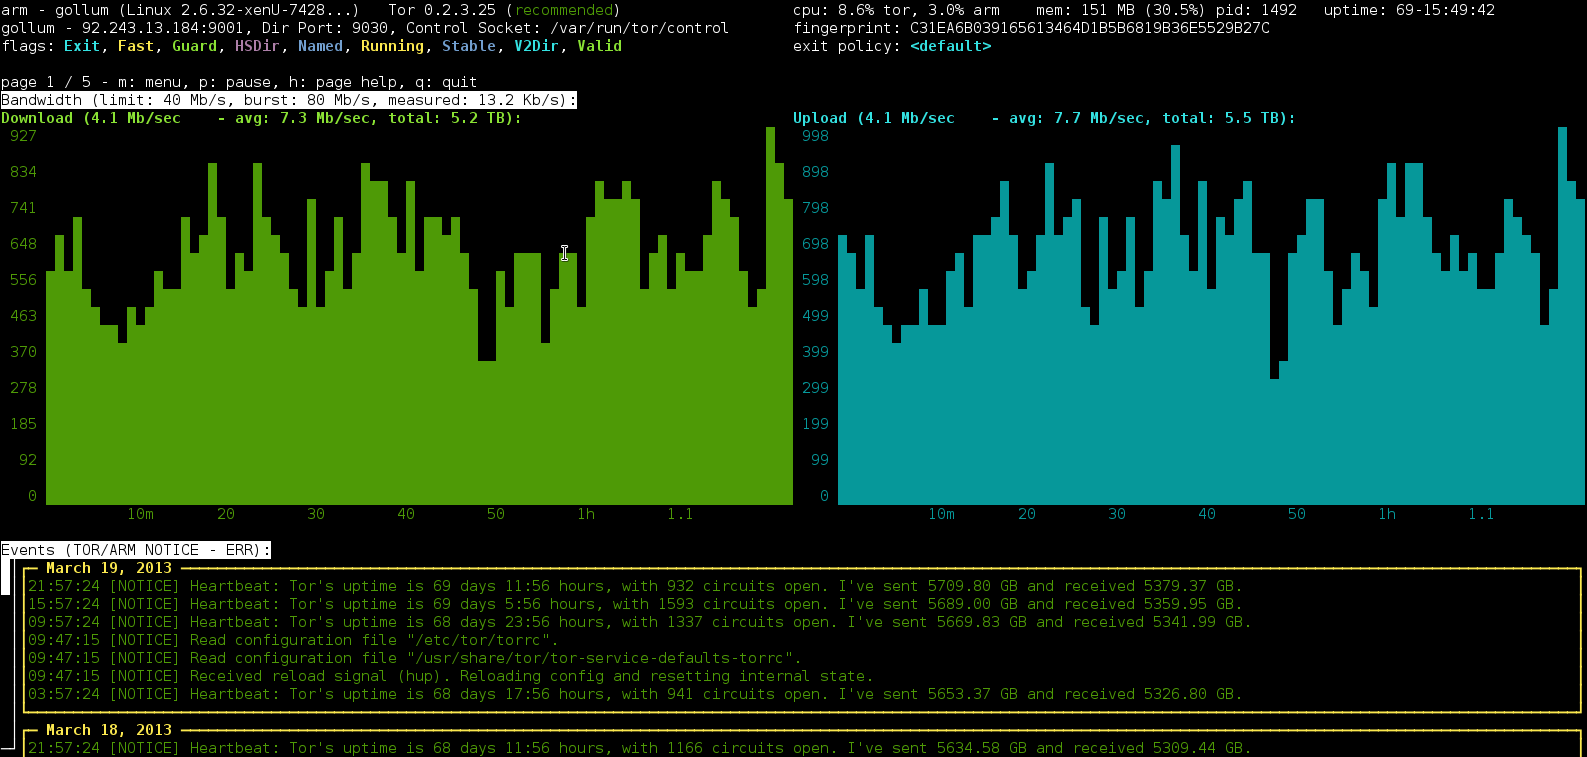
\includegraphics[scale=0.2]{./Multimedia/arm.png}}
	\end{center}
\end{frame}

\begin{frame}[fragile]{Otras webs de monitorización de la red}
	\begin{center}
		\href{https://torstatus.blutmagie.de}{\includegraphics[width=9cm,height=3cm]{./Multimedia/tor_status.png}}
		\\
		Tor Status
		\\
		\vspace{15px}
		\href{https://torflow.uncharted.software/}{\includegraphics[width=9cm,height=3cm]{./Multimedia/tor_flow.png}}
		\\
		Tor Flow
	\end{center}
\end{frame}

\section{Demo Tor Browser}

\begin{frame}[fragile]{¿Qué es el Tor Browser?}
	\pause
	\metroset{block=fill}
	\begin{block}{Tor Browser}
		Es una modificación del navegador Mozilla Firefox de código libre que configura automáticamente el acceso del usuario a la red Tor.
	\end{block}
	\pause
	\begin{alertblock}{Ventajas del Tor Browser}
		Gracias a este navegador los usuarios sin conocimiento acerca de la red pueden utilizarla. Distribuciones como Tails traen este navegador por defecto.
	\end{alertblock}
\end{frame}

\section{Conclusiones}

\begin{frame}[fragile]{Conclusiones}
	\pause
	El anonimato en la red es algo importante y debemos ser conscientes de ello.
	\pause
	\newline
	'Argumentar que no te importa el derecho a la privacidad porque no tienes nada que esconder es como decir que no te importa la libertad de expresión porque no tienes nada que decir.'
	\newline
	Edward Snowden
\end{frame}

\begin{frame}[standout]
	¿Preguntas?
\end{frame}
	
\end{document}